% ::setlocal makeprg=cd\ latex\ &&\ pdflatex\ -interaction=batchmode\ main.tex\ &&\ xdg-open\ main.pdf\ &&\ exit

As we have seen in the previous chapter, the Schwarzschild metric describes the
geometry of spacetime around a spherically symmetric, non-rotating black hole.
Even though it is one of the simplest solutions to the Einstein field equations,
the orbits of particles, in general, are not described by closed form solutions.

In this chapter we will build a program in \texttt{C} that numerically
integrates the equations of motion.
The program will allow us to study more complex geodesics and better understand
how they differ from the Newtonian case.


\section{Equations of motion}
\label{cap2:sec:eq_of_motion}

Recalling the results of the previous chapter we can rewrite the equation for
the radial motion \ref{cap1:eq:like_newton}, together with the equations for
$\phi$ and $t$ that come directly from the conservation of angular momentum and
energy per rest mass unit, respectively eq. \ref{cap1:eq:conserved_l} and
\ref{cap1:eq:conserved_e}.

\begin{subequations}
\label{cap2:eq:eq_of_motion}
	\begin{align}[left = {\empheqlbrace}]
        &\frac{1}{2} \left(\dv{r}{\tau}\right)^2 = \mathcal E - V_{\rm eff} (r)
        \\
        &\dv{\phi}{\tau} = \frac{l}{r^2} \\
        &\dv{t}{\tau} = \frac{e}{1 - 2 M / r}
	\end{align}
\end{subequations}

Where $V_{\rm eff}$ is the effective potential defined in eq.
\ref{cap1:eq:V_eff} and $\mathcal E = \frac{e^2 - 1}{2}$.

To avoid numerical problems, we will keep geometrized units and express
everything in unit of the \Sh radius $r_s = 2 M$:

\begin{equation}
    r = r_s \hat r \quad \quad
    \tau = r_s \hat \tau \quad \quad
    t = r_s \hat t \quad \quad
    \ell = r_s \hat \ell \quad \quad
\end{equation}

The system of equations \ref{cap2:eq:eq_of_motion} can be rewritten as

\begin{subequations}
    \begin{align}[left = {\empheqlbrace}]
        &\dv{\hat r}{\hat \tau} = \pm \sqrt{2 \mathcal E - 2 V_{\rm eff}}
        \label{cap2:eq:radial_eq_as} \\
        &\dv{\phi}{\hat \tau} = \frac{\hat \ell}{\hat r^2}
        \label{cap2:eq:angular_eq_dimless} \\
        &\dv{t}{\hat \tau} = \sqrt{2 \mathcal E + 1}
        \left(\frac{\hat r}{\hat r - 1}\right) \label{cap2:eq:time_eq_dimless}
    \end{align}
    \label{cap2:eq:eq_of_motion_ad}
\end{subequations}

The effective potential becomes

\begin{equation}
    V_{\rm eff} = \frac{1}{2} \left(\frac{\hat \ell^2}{\hat r^2}
    - \frac{1}{\hat r} - \frac{\hat \ell^2}{\hat r^3} \right) \, .
\end{equation}

The condition on the angular momentum $\ell$ for the existence of a stable
orbits is $\ell > \sqrt{12} M$ and becomes $\hat \ell > \sqrt{3}$.
The stationary points of $V_{\rm eff}$ from eq. \ref{cap1:eq:V_eff} are

\begin{subequations}
    \begin{align}
        \hat r_{\substack{\text{min} \\ \text{max}}} &= \hat \ell^2
        \left(1 \pm \sqrt{1 - \frac{3}{\hat \ell^2}} \right)
        &&{\rm for} \quad \hat \ell > \sqrt{3} \\
        \hat r_{\rm ISCO} &= 3
        &&{\rm for} \quad \hat \ell = \sqrt{3}
    \end{align}
\end{subequations}

Where $\hat r_{\substack{\text{min} \\ \text{max}}}$ respectively represent a
local minimum and maximum of the effective potential.
The system in \ref{cap2:eq:eq_of_motion_ad} can be solved numerically with
a fourth-order \texttt{Runge-Kutta} method.
The initial conditions that determine the orbit are $\hat \ell$,
$\mathcal E$ and a compatible starting radius $\hat r_0$ (refer to Figure
\ref{cap1:fig:V_eff_orbits}).

To find the range of $r$ that the particle can explore we need to study when the
argument of the square root in eq. \ref{cap2:eq:radial_eq_as} is positive.
In general, we need to solve a cubic equation

\begin{equation}
    \dv{\hat r}{\hat \tau} = 0
    \quad \Rightarrow \quad
    \mathcal E - V_{\rm eff} = 0
    \quad \Rightarrow \quad
    \hat r^3 - \hat \ell^2 \hat r^2 + \hat \ell^2 - 2 \mathcal E
    \hat r - \hat \ell^2 = 0 \, .
    \label{cap2:eq:cubic_eq}
\end{equation}

All the possible scenarios are resumed in Table \ref{cap2:tab:scenarios}.

\begin{table}[h]
    \centering
    \begin{tabular}{cccc}
        $\hat \ell$     & $\mathcal E$                  & $\hat r$     
                                                        & Scenario \\
        $[0,~\sqrt{3}]$ & $[0,~\infty]$                 & $(1,~\infty)$
                                                        & depends on the sign\\
        $[0,~\sqrt{3}]$ & $[-\frac{1}{2},~0]$           & $(1,~r_e)$   
                                                        & infall \\
        $(\sqrt{3},~2]$ & $[0,~\infty]$                 & $(1,~\infty)$ 
                                                        & depends on the sign \\
        $(\sqrt{3},~2]$ & $[V_{\rm max},~0]$            & $(1,~r_2)$
                                                        & infall \\
        $(\sqrt{3},~2]$ & $[V_{\rm min},~V_{\rm max}]$  & $(r_1,~r_2)$
                                                        & bound orbit \\
        $(\sqrt{3},~2]$ & $[-\frac{1}{2},~V_{\rm min}]$ & $(1,~r_e)$
                                                        & infall \\
        $(2, \infty)$   & $[V_{\rm max},~\infty]$       & $(1,~\infty)$ 
                                                        & depends on the sign \\
        $(2, \infty)$   & $[0,~V_{\rm max}]$            & $(r_1,~\infty)$
                                                        & unbound orbit \\
        $(2, \infty)$   & $[V_{\rm min},~V_{\rm min}]$  & $(r_1,~r_2)$
                                                        & bound orbit \\
        $(2, \infty)$   & $[-\frac{1}{2},~V_{\rm min}]$ & $(1,~r_e)$
                                                        & infall \\
    \end{tabular}
    \caption{Possible scenarios for the motion of a particle in the \Sh
    spacetime.}
    \label{cap2:tab:scenarios}
    %% A Figure would probably be better
\end{table}

In the table we referred to the local maximum and minimum of the effective
potential calculated in $r_{\substack{\text{min} \\ \text{max}}}$ as
$V_{\rm min}$ and $V_{\rm max}$ respectively.
Instead of solving the cubic equation analytically, the limiting radii can be
calculated using the bisect method and imposing that \ref{cap2:eq:cubic_eq}
must be 0 between 1 and $r_{\rm min}$ for $r_e$, between $r_{\rm min}$ and
$r_{\rm max}$ for $r_1$ and between $r_{\rm max}$ and $\infty$ (1000 in our
case) for $r_2$.

%% NON MI PIACE

%% HOW TO CHANGE SIGN
\newpage


\section{Infalls}

Similarly to the previous chapter, we can start with a radial infall scenario,
where $\hat \ell = 0$, $\mathcal E = 0$.

\begin{figure}[h]
    \begin{minipage}{0.48\textwidth}
        \centering
        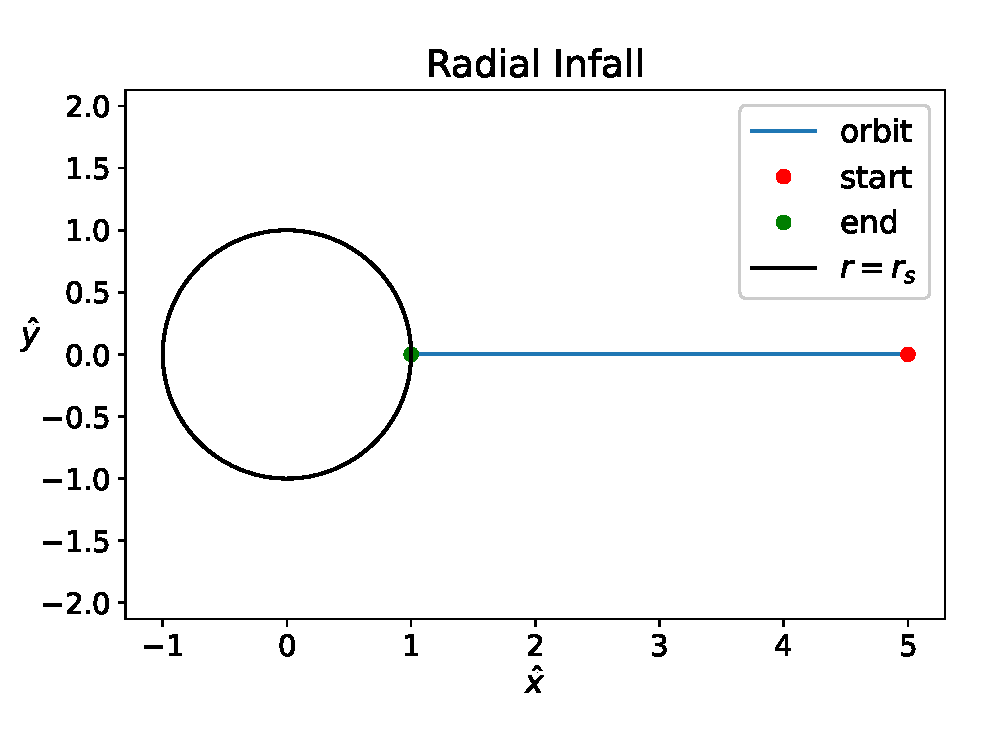
\includegraphics[width=\textwidth]{Figures/chapter2/radial_infall.eps}
        \caption{Plot of the orbit of a particle in radial infall ($\hat \ell = 0$
        and $\mathcal E = 0$). \\}
    \end{minipage}
    \hspace{0.015 \textwidth}
    \begin{minipage}{0.48\textwidth}
        \centering
        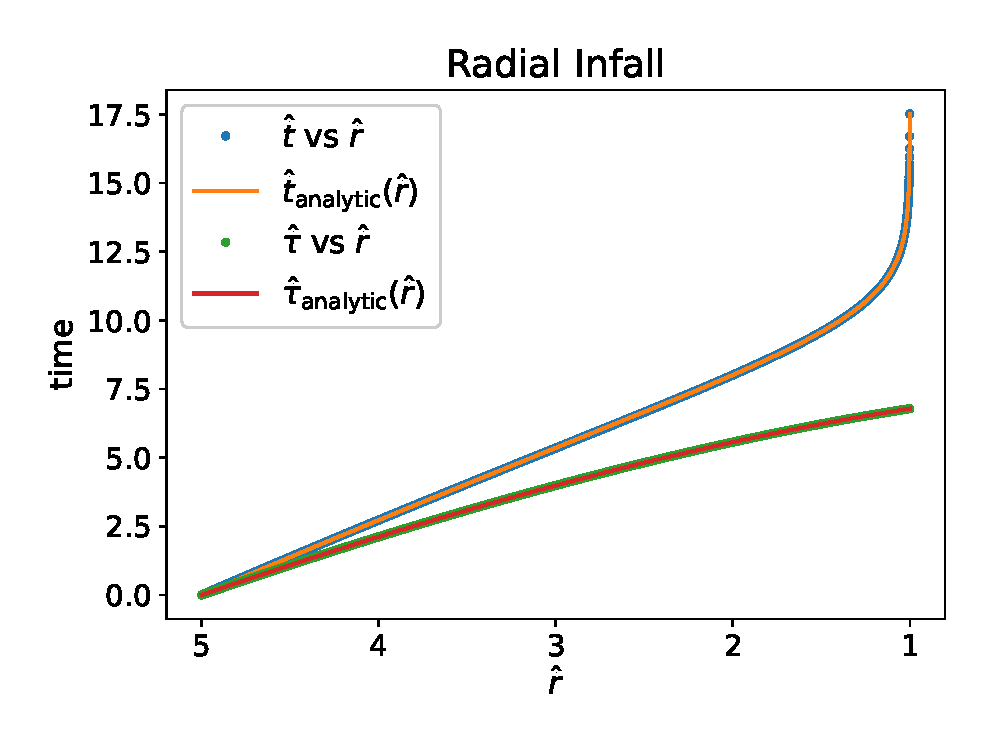
\includegraphics[width=\textwidth]{Figures/chapter2/t_vs_tau.eps}
        \caption{Proper time against \Sh time with respect of the radius of a
        particle falling towards $r = r_s$.}
    \end{minipage}
\end{figure}

The orbit plot is not the most interesting, but the time plot shows that the
numerical integration is working correctly, as the results are consistent with
eq. \ref{cap1:eq:radial_infall_r_of_tau} and \ref{cap1:eq:radial_infall_r_of_t}
found analytically in the previous chapter. \\
Figures \ref{cap2:fig:t_res} and \ref{cap2:fig:tau_res} also show the residuals
of $\hat t$ and $\hat \tau$ with respect to their analytical predictions.
For $\hat \tau$ the error is of the order of $10^{-10}$.
For $\hat t$ the vertical axis is in logarithmic scale to show that the error is
constant around $10^{-10}$ only to increase when the particle gets closer to the
\Sh radius.
That's to be expected as $t \rightarrow \infty$ when $r \rightarrow r_s$.

\begin{figure}[h]
    \begin{minipage}{0.48\textwidth}
        \centering
        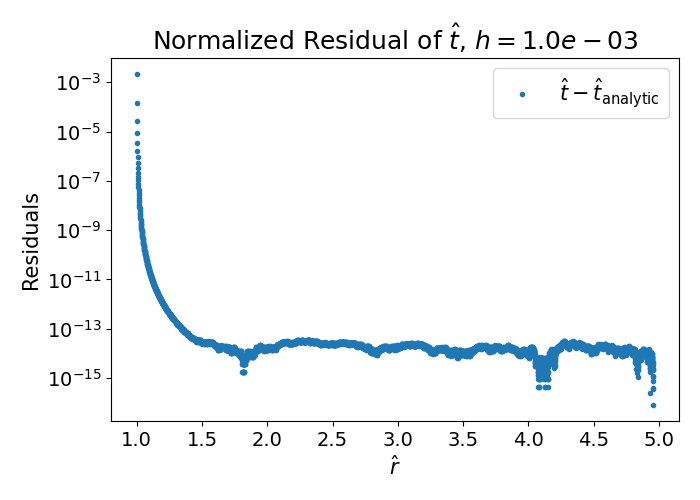
\includegraphics[width=\textwidth]{Figures/chapter2/t_res.png}
        \caption{Residual plot of $\hat t$ against the analytical prediction
        found in eq. \ref{cap1:eq:radial_infall_r_of_t}.}
        \label{cap2:fig:t_res}
    \end{minipage}
    \hspace{0.015 \textwidth}
    \begin{minipage}{0.48\textwidth}
        \centering
        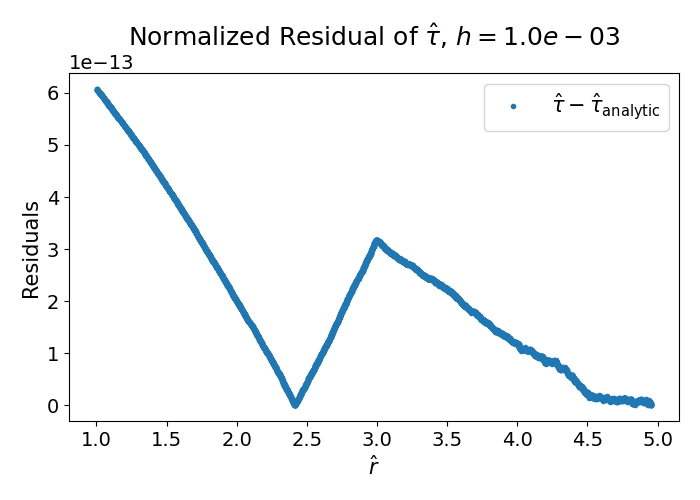
\includegraphics[width=\textwidth]{Figures/chapter2/tau_res.png}
        \caption{Residual plot of $\hat \tau$ against the analytical prediction
        found in eq. \ref{cap1:eq:radial_infall_r_of_tau}.}
        \label{cap2:fig:tau_res}
    \end{minipage}
\end{figure}

By integrating numerically with this program, we can visualize some more
complex infalls that are shown in Figures \ref{cap2:fig:infall1} and
\ref{cap2:fig:infall2}.

\begin{figure}[h!]
    \begin{minipage}{0.48\textwidth}
        \centering
        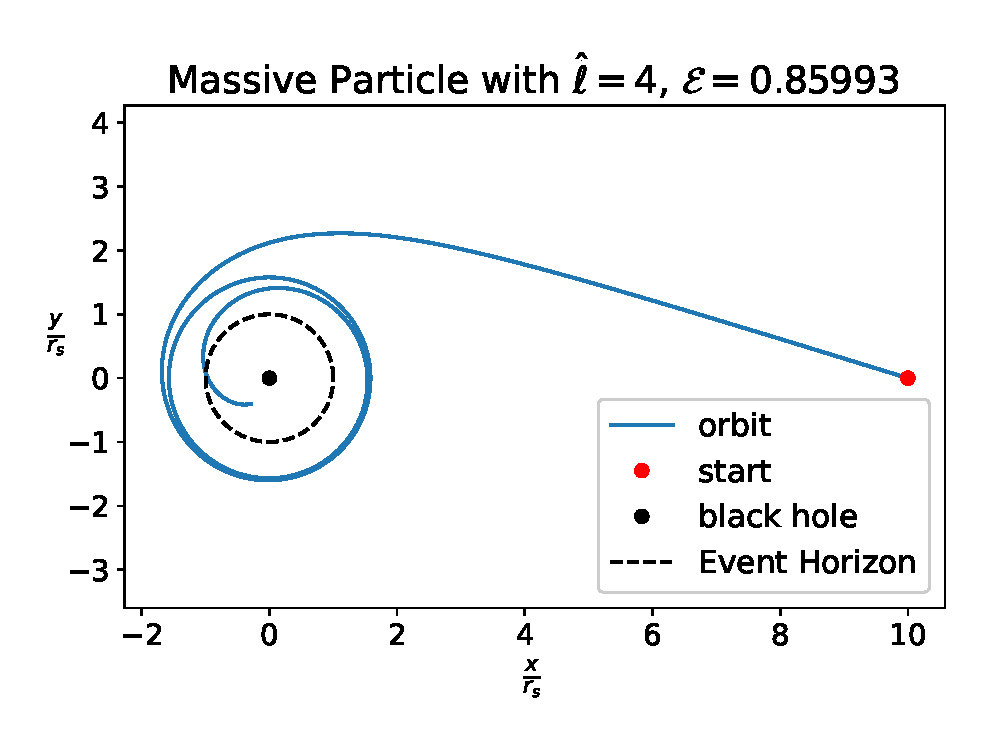
\includegraphics[width=\textwidth]{Figures/chapter2/infall1.eps}
        \caption{The particle starts at $\hat r_0 = 10$
        ($\hat r_{\rm max} \simeq 1.6$) and has an energy slightly greater than
        $V_{\rm eff}(r_{\rm max}) \simeq 0.859927$.
        As a result the radial velocity decreases when the particle passes
        through $\hat r = \hat r_{\rm max}$.}
        \label{cap2:fig:infall1}
    \end{minipage}
    \hspace{0.015 \textwidth}
    \begin{minipage}{0.48\textwidth}
        \centering
        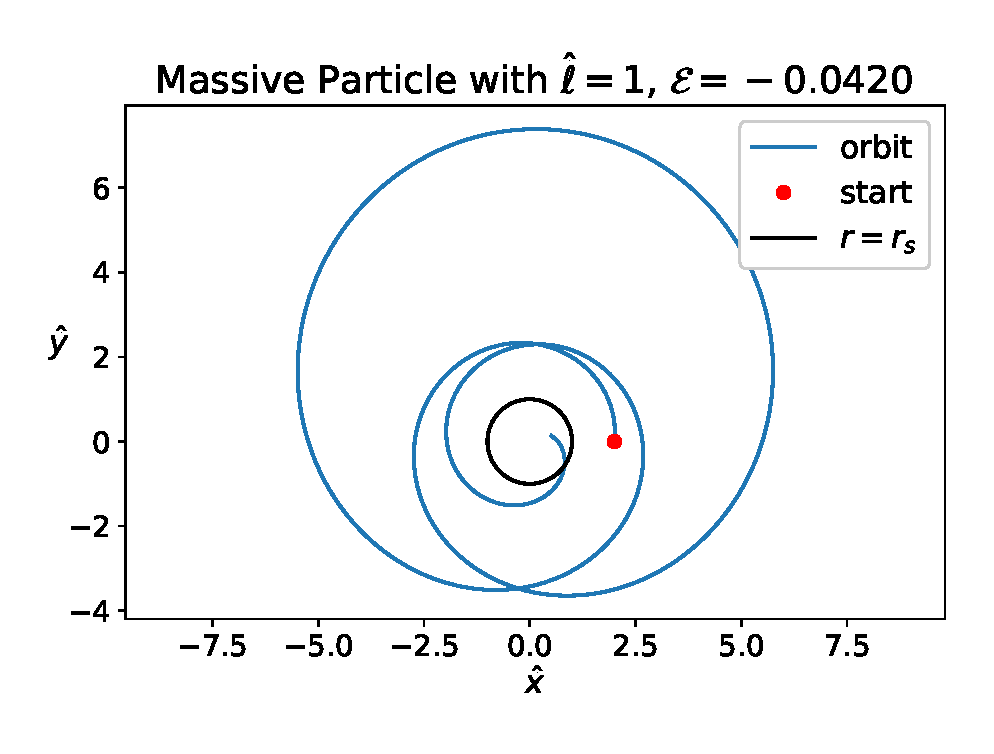
\includegraphics[width=\textwidth]{Figures/chapter2/infall2.eps}
        \caption{$V_{\rm eff}$ is monotonic because $\ell < \sqrt{3}$.
        The particle starts at $\hat r = 2$ with its radial velocity
        directed outward; however, due to its negative energy $\mathcal E$, the
        particle will not be able to escape.}
        \label{cap2:fig:infall2}
    \end{minipage}
\end{figure}


\section{Bound Orbits}

\subsection{Circular Orbits}

We can also study bound orbits when considering particles with
$\hat \ell > \sqrt{3}$ and $\mathcal E < \min \{V_{\rm max}, 0\}$.
As seen in section \ref{cap1:ssec:circular_orbits} in the previous chapter we
have a circular orbit only if $\mathcal E = V_{\rm eff}({\rm min})$.
In this case holds the relation (from eq. \ref{cap1:eq:Omega2})

\begin{equation}
    \Omega^2 = \frac{1}{2 \hat r^3}
    \quad \quad \quad {\rm where} \quad \quad \quad
    \Omega := \dv{\phi}{\hat t} \, .
\end{equation}

In Figure \ref{cap2:fig:circ_orbit} we can see the orbit of a particle with
$\hat \ell = 3$ and $\mathcal E = V_{\rm eff}(r_{\rm min}) \simeq
\num{-1.478e-02}$.
Figure \ref{cap2:fig:circ_orbit_res} shows the normalized residuals of the
angular velocity $\Omega$ computed from $\phi$ and $\hat t$ obtained during the
simulation against the expected value.

\begin{figure}[h]
    \begin{minipage}{0.48\textwidth}
        \centering
        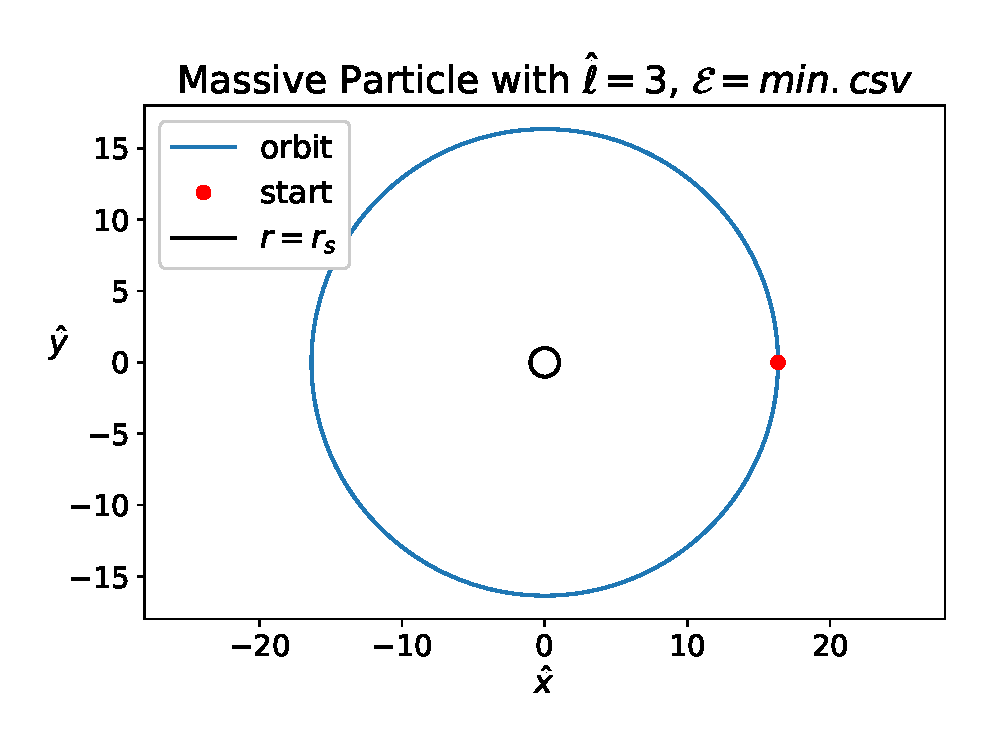
\includegraphics[width=\textwidth]{Figures/chapter2/circ.eps}
        \caption{The perfectly circular orbit of a particle with $\hat \ell = 3$
        and $\mathcal E = V_{\rm eff}(r_{\rm min}) \simeq \num{-1.478e-02}$.
        The particle starts at $\hat r = r_{\rm min} \simeq 16.35$ and the
        radius is left unchanged.}
        \label{cap2:fig:circ_orbit}
    \end{minipage}
    \hspace{0.015 \textwidth}
    \begin{minipage}{0.48\textwidth}
        \centering
        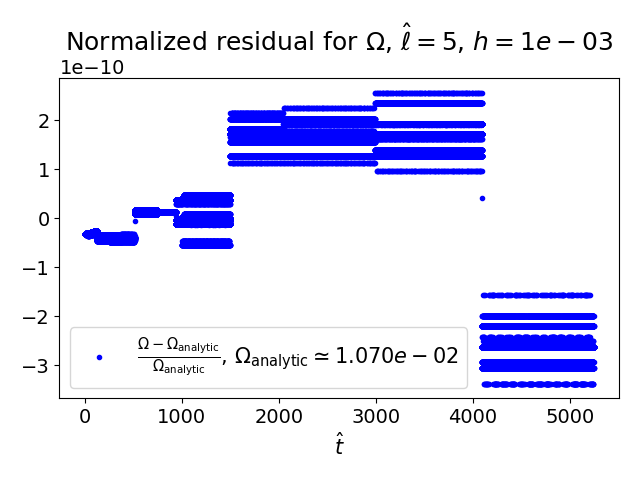
\includegraphics[width=\textwidth]{Figures/chapter2/circular_orbit_res.png}
        \caption{The residual of the calculated angular velocity $\Omega$ from the
        data of $\phi$ and $\hat t$ and the expected value calculated from the
        initial radius $\Omega_{\rm analytic} = 1 / (2 \hat r_{\rm min})$.}
        \label{cap2:fig:circ_orbit_res}
    \end{minipage}
\end{figure}

The relative error is of order $10^{-10}$ with a time increment $h = 0.001$, we
can conclude that the numerical integration is correctly implemented and most
of the error comes from the finite precision.


\subsection{Precession}

Therefore, we can proceed with confidence to study bound orbits of different
shapes.
Recall from eq. \ref{cap1:eq:precession} and \ref{cap1:eq:delta_phi} that, for a
bound orbit where the two turning points are labeled $r_1 < r_2$, the
precession is given by

\begin{equation}
    \delta \phi = 2 \int_{r_1}^{r_2} \left( 2 \mathcal E + \frac{2M}{r}
    - \frac{l^2}{r^2} + \frac{2Ml^2}{r^3} \right)^{-1/2} \, \dd{r}
    \; - 2 \pi \, .
\end{equation}

If we make the substitution $r = 1 / u$ and use the definition of $\mathcal E
= \frac{e^2 - 1}{2}$, we can rewrite the integral as

\begin{equation}
    \delta \phi = 2 \int_{u_2}^{u_1} \frac{1}{\sqrt{2 \mathcal E + 2Mu - l^2 u^2
    + 2Ml^2 u^3}} \, \dd{u}
    \; - 2 \pi \, .
    \label{cap2:eq:delta_phi}
\end{equation}

The bounds of the integral are $u_2 = 1 / r_2 < u_1 = 1 / r_1$.
Under the square root we have a cubic equation in $u$ with coefficients

\begin{align}
    &{\rm coefficients} && a = 2Ml^2, \quad b = -l^2, \quad c = 2M, \quad d = 2 \mathcal E \\
    &{\rm roots}        && u_1, ~ u_2, ~ u_3 \, .
    \label{cap2:eq:cubic_roots}
\end{align}

Since all the coefficients are real, the roots of the equation must either
consist of three real roots or one real root and a pair of complex conjugate
roots.
Given that we are considering bound orbits, we know that two real roots must
exist.
Therefore, we can infer that all three roots are real and can be labeled such
that $u_1 < u_2 < u_3$.

The Wikipedia article \textit{Precession of orbits} \footcite{enwiki:1242536958}
shows that, knowing the roots in \ref{cap2:eq:cubic_roots}, the integral in
\ref{cap2:eq:delta_phi} can be expressed in terms of the complete elliptic
integral of the first kind $K(m)$

\begin{equation}
    \delta \phi = 2 \int_{u_2}^{u_1} \frac{1}{\sqrt{(u - u_1)(u - u_2)(u - u_3)}}
    \, \dd{u} \; - 2 \pi
    = \frac{K(m)}{\sqrt{r_s (u_3 - u_1)}} - 2 \pi \, .
\end{equation}

Where $K$ and $m$ are respectively defined as

\begin{equation}
    K(m) = \int_0^{\pi/2} \frac{\dd{\theta}}{\sqrt{1 - m \sin^2 \theta}} \, ,
    \quad \quad \quad
    m = \frac{u_2 - u_1}{u_3 - u_1}
\end{equation}

and can be numerically solved in python using the \texttt{scipy.special.ellipk}
function.

We can now compare the precession of a particle computed from the numerical data
of the simulation with the expected value calculated from the initial conditions
with the library for elliptic integrals.

Figure \ref{cap2:fig:prec1} \ref{cap2:fig:prec2}  ref ref
shows some examples of bound orbits with different values of $\hat \ell$ and
$\mathcal E$.

\begin{figure}[h]
    \begin{minipage}{0.48 \textwidth}
        \centering
        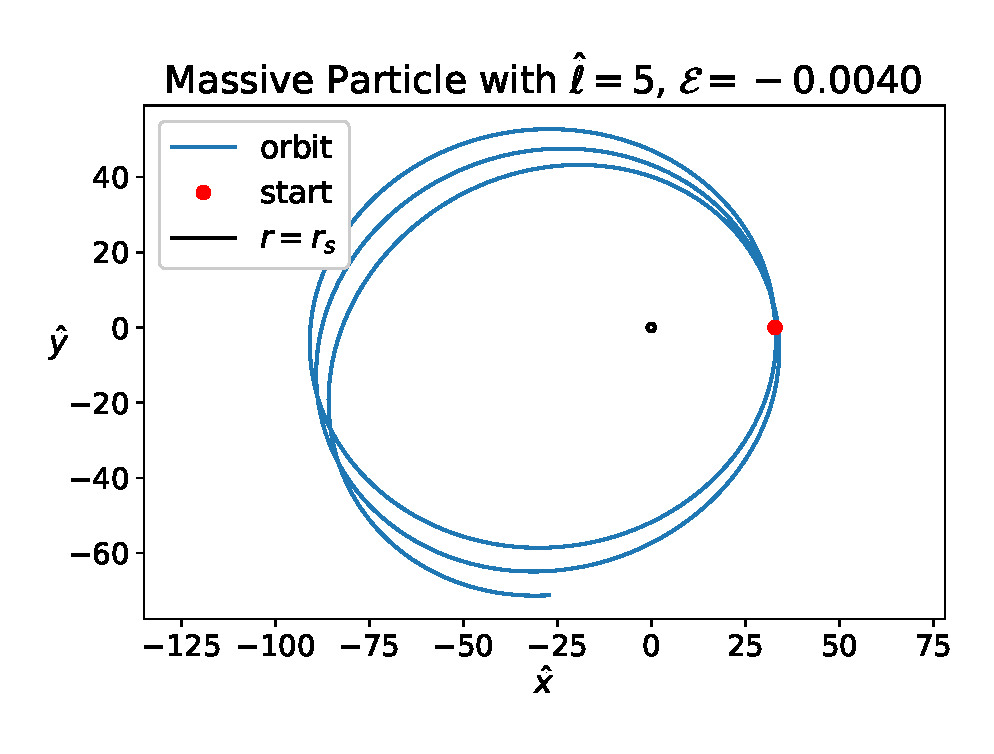
\includegraphics[width=\textwidth]{Figures/chapter2/prec1.eps}
        \caption{$\hat \ell = 5$ produces a local minimum $V_{\rm eff}
        (r_{\rm min}) \simeq = -0.0051$, }
        \label{cap2:fig:prec1}
    \end{minipage}
    \hspace{0.015 \textwidth}
    \begin{minipage}{0.48 \textwidth}
        \centering
        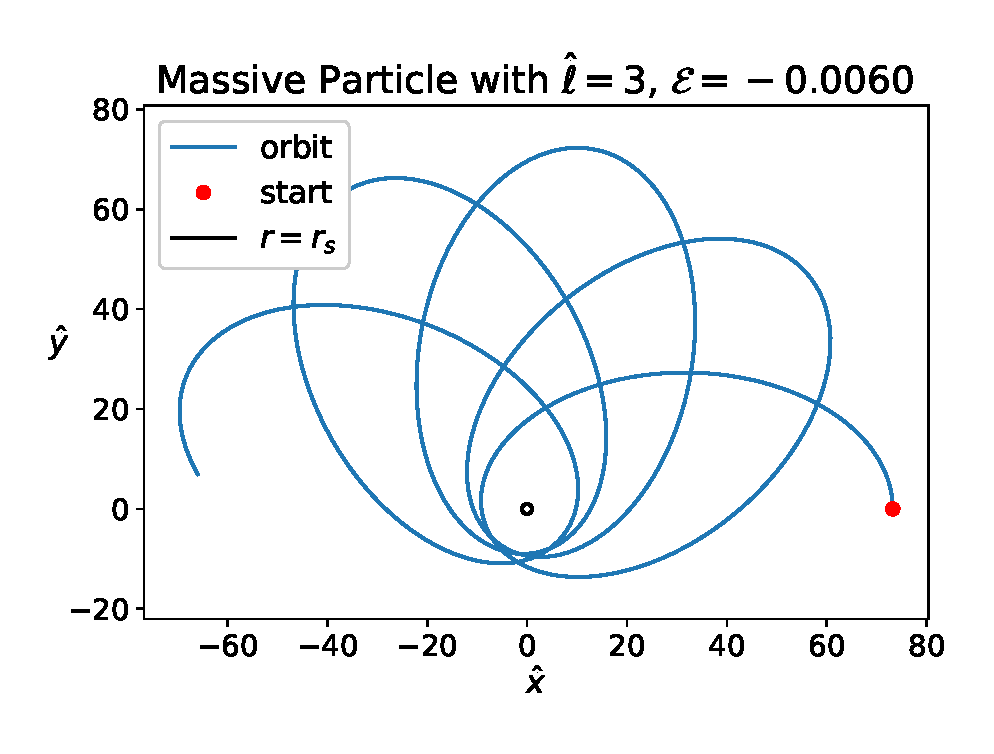
\includegraphics[width=\textwidth]{Figures/chapter2/prec2.eps}
        \caption{}
        \label{cap2:fig:prec2}
    \end{minipage}
\end{figure}
